\mysection{РАЗРАБОТКА ПРИЛОЖЕНИЯ}

\subsection{Подготовка окружения для разработки}

Основой разрабатываемого приложения является JavaScript-фреймворк Vue.js. Данный фреймворк позволяет начать работу над проектом максимально просто -- достаточно добавить на веб-страницу JavaScript-файл с~кодом Vue.js, используя HTML-тег \emph{script}.

Однако, для обеспечения удобства разработки и~возможности использования новейших возможностей языка JavaScript было решено использовать пакетный менеджер NPM \cite{NPM} вместе с~компилятором Babel \cite{Babel} и~утилитой Webpack \cite{Webpack}, предназначенной для сборки веб-приложений.


\subsubsection{Пакетный менеджер NPM}

\textbf{NPM} (аббр. \emph{Node Package Manager}) -- менеджер пакетов, входящий в~состав программной платформы Node.js \cite{NodeJS}. NPM существенно упрощает установку компонентов, необходимых для работы или сборки приложения.

При работе с~данным пакетным менеджером, особый интерес представляет файл \textbf{package.json}. Данный файл содержит информацию о~разрабатываемом приложении: название, версия, описание и~т.д (см. листинг \ref{lst:package_json}). Но наиболее важным содержимым файла package.json являются зависимости -- список имён и~версий пакетов, требующихся для работы приложения.


\subsubsection{Babel}

\textbf{Babel} -- транспилер (англ. \emph{transpiler}), транслирующий код JavaScript стандартов ES2015 и~новее \cite{ecma262} в~код более ранних версий JavaScript.

Применение данного инструмента при разработке проекта позволяет использовать возможности JavaScript, представленные в~новейших стандартах языка, не теряя при этом совместимость приложения со~старыми версиями веб-браузеров.

% TODO Пример работы Babel
% TODO Список поддерживаемых браузеров?
\lstinputlisting[
  caption={Пример содержимого файла package.json},
  label={lst:package_json}
]{src/package.json}


\subsubsection{Webpack}

\textbf{Webpack} -- система сборки для JavaScript-приложений, предназначенная, в первую очередь, для генерирования статических ресурсов на основе JavaScript-модулей и~их зависимостей.

Одним из основных преимуществ Webpack является его способность работать с~практически любыми типами ресурсов. Данная возможность обеспечивается дополнительно устанавливаемых \emph{загрузчиков} (англ. \emph{loaders}), которые, к~примеру, позволяют:
\begin{dashitemize}
  \item производить компиляцию JavaScript-файлов с~помощью Babel;
  \item осуществлять статический анализ кода с~помощью ESLint \cite{ESLint};
  \item минифицировать и обфусцировать код приложения;
  \item обрабатывать файлы с~расширением <<.vue>> (однофайловые компоненты Vue.js);
  \item производить трансляцию стилей, описанных на языке SCSS \cite{Sass}, в~CSS.
\end{dashitemize}

Стоит также отметить, что с~помощью Webpack можно существенно облегчить разработку веб-приложения. Благодаря специальным расширениям становится возможно запустить локальный HTTP-сервер, позволяющий просматривать и~отлаживать разрабатываемое приложение в~браузере компьютера, на котором ведётся разработка.



\subsection{Структура проекта}

Исходный код клиентской части приложения является частью Python-проекта, написанного с использованием веб-фреймворка Flask. Подобная структура проекта позволяет держать весь код приложения в одном репозитории и облегчает сборку Python-приложения, предназначенного для установки на устройства Reach и~Reach~RS.

Код клиентского веб-приложения находится в директории \emph{static-src}. Структура данной директории подробно описана на рисунке \ref{fig:project-tree}.

\begin{figure}[h!]
  \centering
  \setlength{\fboxsep}{5pt}
  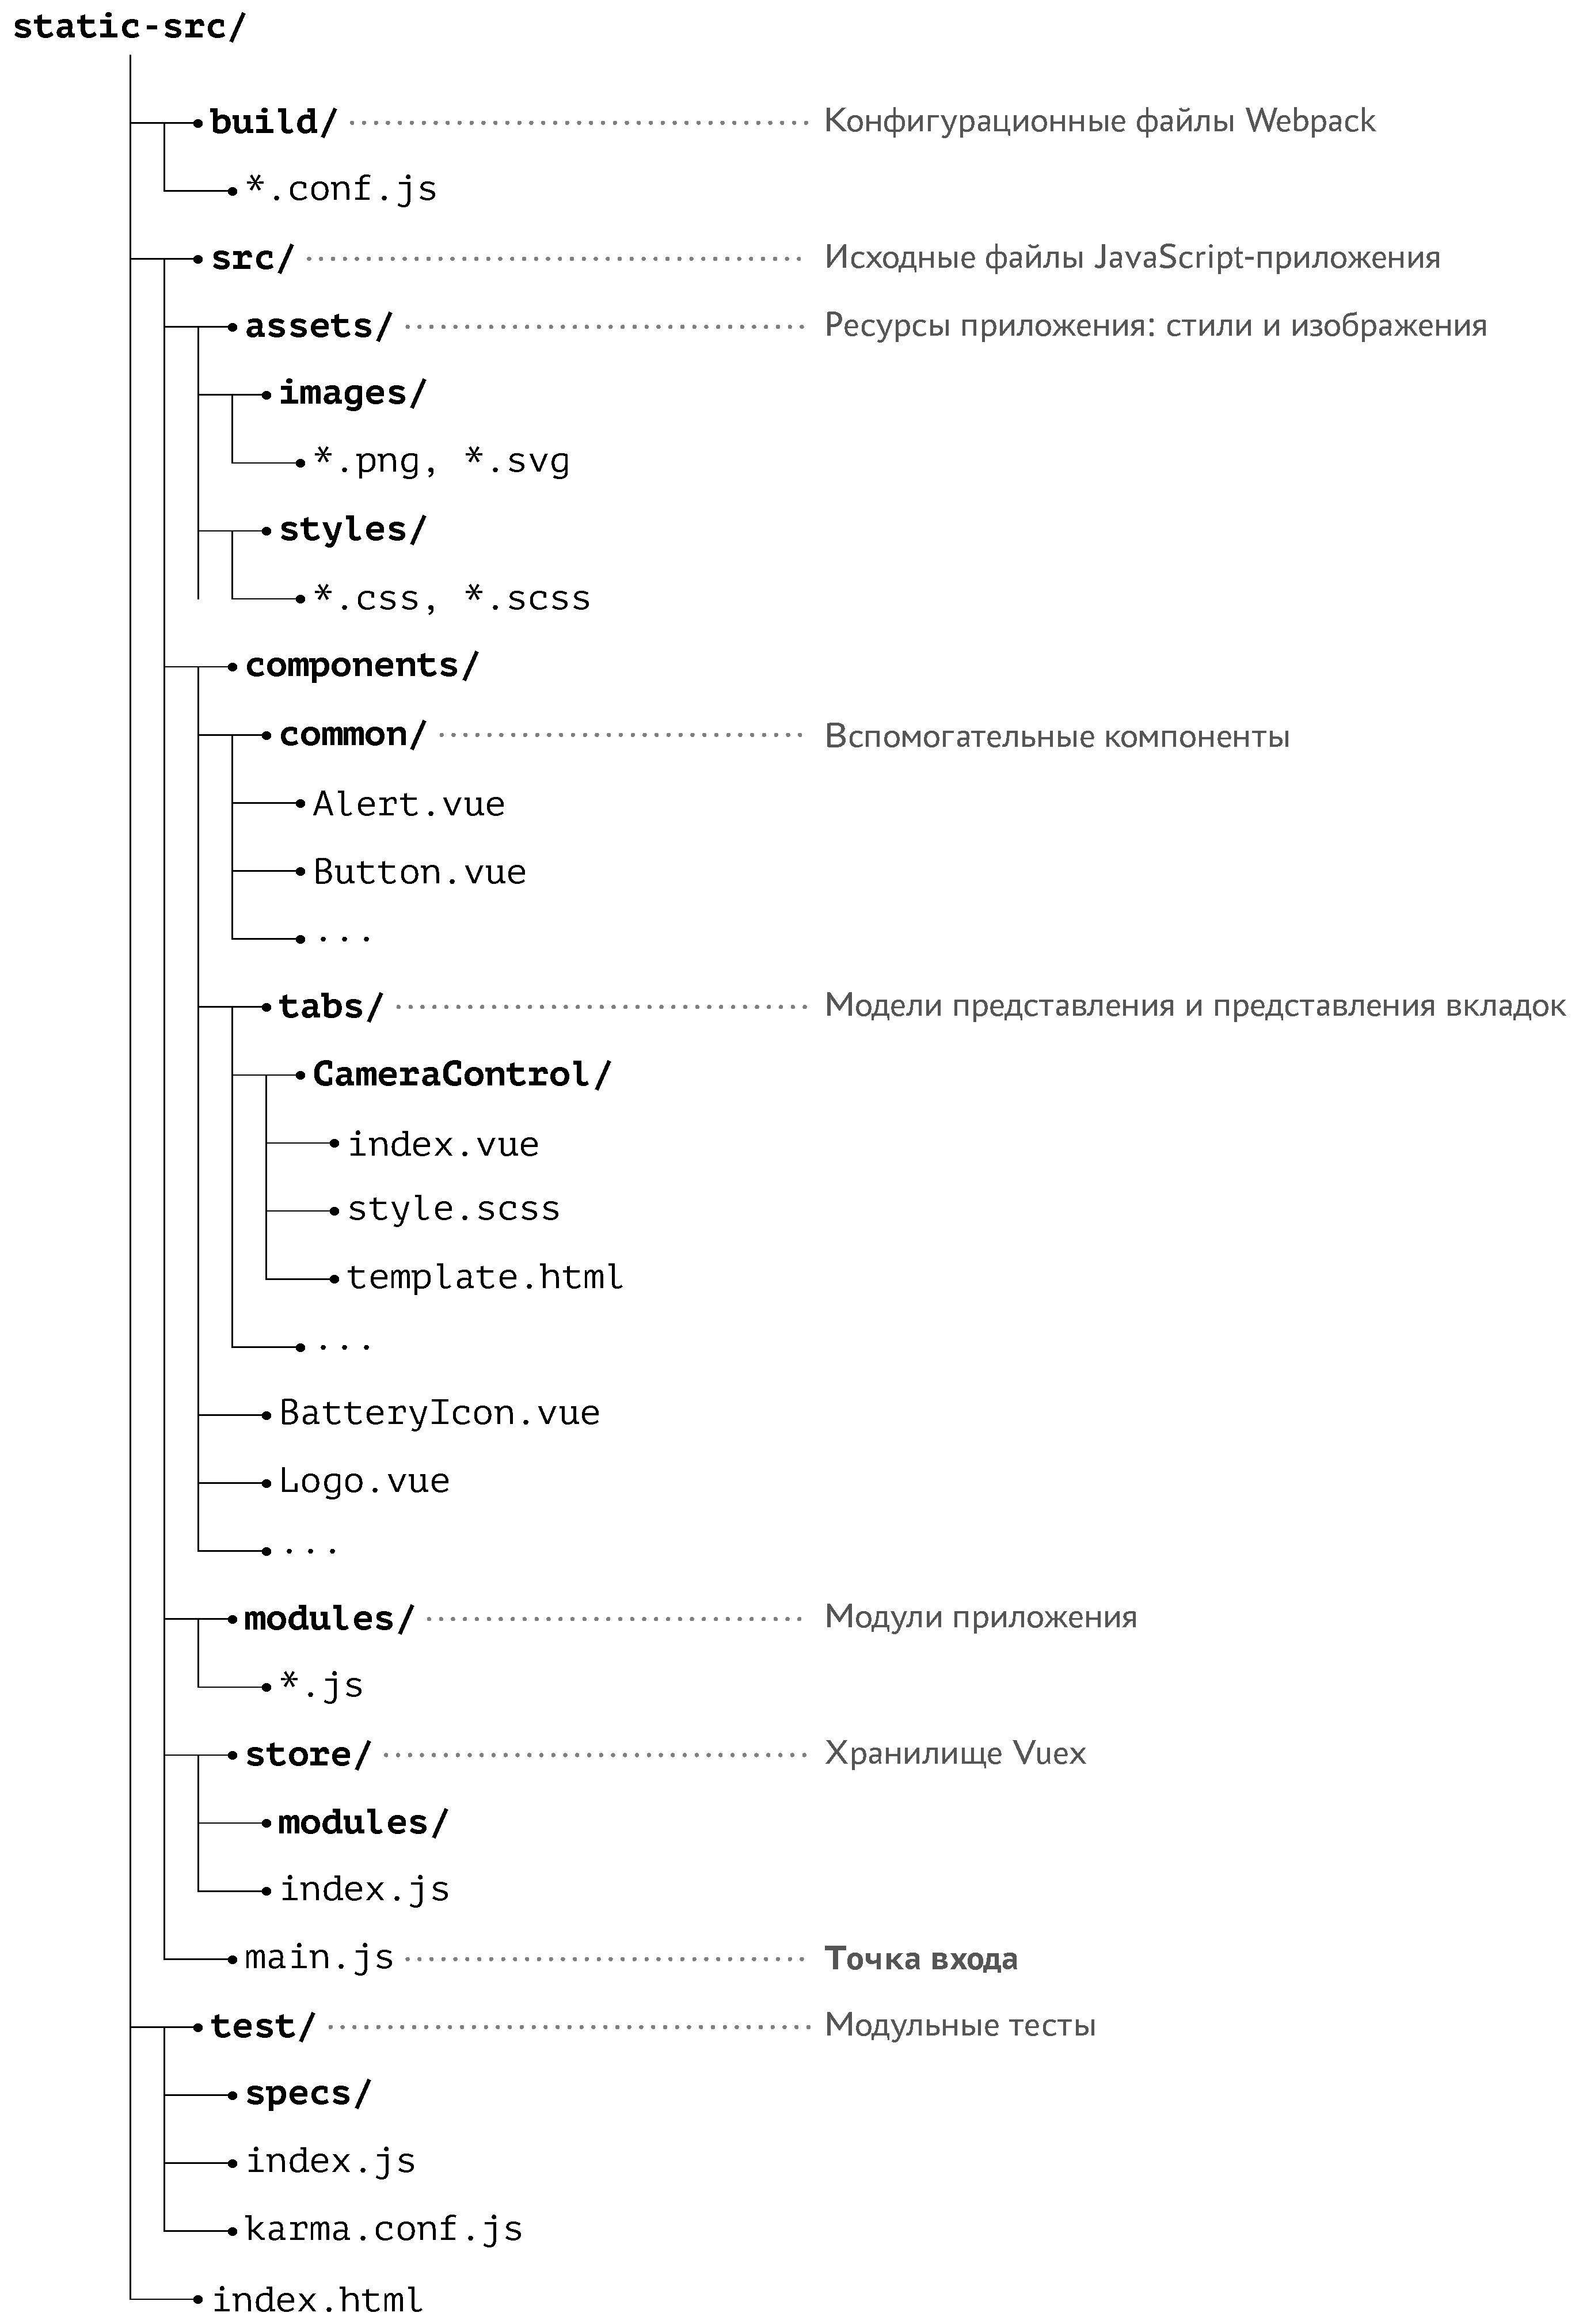
\includegraphics[width=.95\textwidth]{img/tikz/project-tree/pic}
  \vspace*{6pt}
  \caption{Структура проекта}\label{fig:project-tree}
\end{figure}



\subsection{Глобальное хранилище данных приложения. Однонаправленный поток данных}

\textbf{Vuex} -- библиотека-расширение для Vue.js приложений, позволяющая создавать глобальное хранилище данных, доступное для всех модулей и Vue-компонентов, входящих в~состав проекта. Подобное хранилище необходимо не только для обмена данными между компонентами -- основной его задачей является управление состоянием представлений приложения.

Идеи, лежащие в~основе данной библиотеки, унаследованы от архитектуры Flux \cite{Flux}. Vuex предоставляет шаблонный подход к~управлению состояниями компонентов приложения, основанный на \emph{однонаправленном потоке данных}.


\subsubsection{Однонаправленный поток данных}

Взаимный обмен данными и~событиями между моделями и~представлениями при наличии большого числа компонентов является потенциальным источником ошибок. Асинхронные изменения и~побочные эффекты могут существенно усложнить разработку и~отладку, а~также нарушить работу приложения.

% TODO Добавить "переход" к этому абзацу
Однонаправленный поток данных в~простейшем виде представлен на рисунке \ref{fig:simple-oneway-data-flow}.

\begin{figure}[h!]
  \centering
  \setlength{\fboxsep}{5pt}
  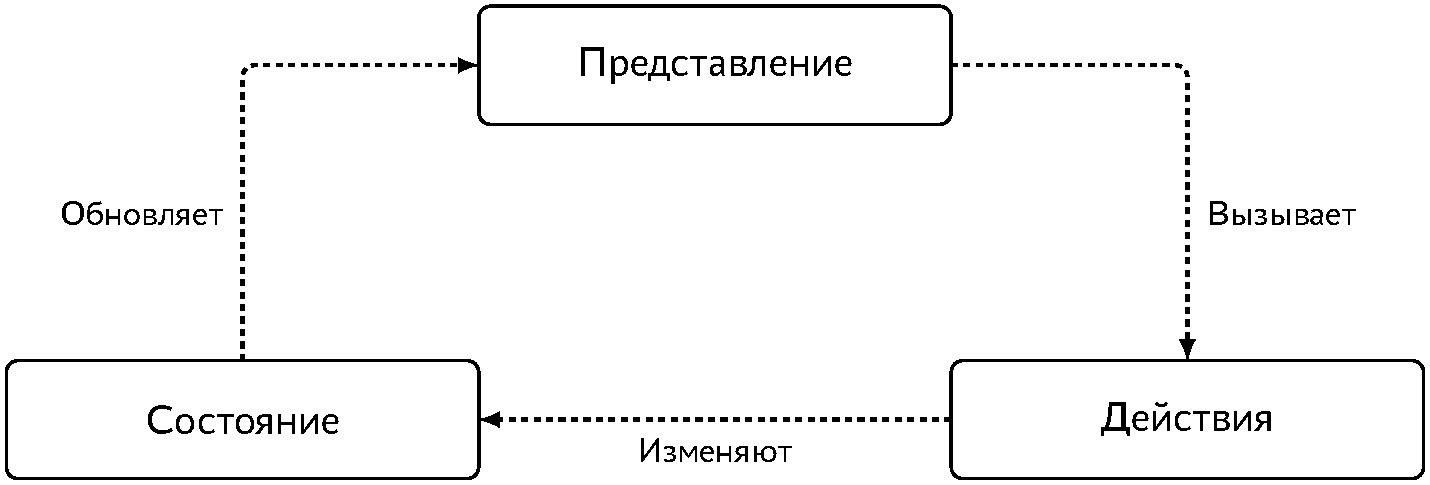
\includegraphics[width=.9\textwidth]{img/tikz/simple-oneway-data-flow/pic}
  \vspace*{12pt}
  \caption{Однонаправленный поток данных}\label{fig:simple-oneway-data-flow}
\end{figure}

\newpage

Подход, описанный на рисунке \ref{fig:simple-oneway-data-flow}, прекрасно подходит для управления представлением одного компонента. Однако, при появлении нескольких компонентов, зависящих от одного и~того же состояния, структура приложения может существенно усложниться.

% TODO Сноска про <<одиночку>>?
Vuex решает проблему, описанную выше, вводя в~структуру приложения глобальное хранилище данных, являющееся состоянием-<<одиночкой>> (англ. \emph{singleton}), которое обновляет все необходимые представления с~помощью реактивных обновлений.

Для избежания неконтролируемых изменений состояния в~Vuex введено следующее ограничение: изменить состояние можно только с~помощью синхронных транзакций, называемых \emph{мутациями}.

Асинхронные операции, результаты выполнения которых изменяют состояние, в~Vuex получили название \emph{<<действия>>}. Внутри функций-обработ-чиков действий становится возможно, к~примеру, совершить асинхронный запрос к~серверу, а~при получении результата сделать одну или более синхронных мутаций состояния.

Схема организации однонаправленного потока данных при использовании Vuex изображена на рисунке \ref{fig:vuex-oneway-data-flow}.

\begin{figure}[h!]
  \centering
  \setlength{\fboxsep}{5pt}
  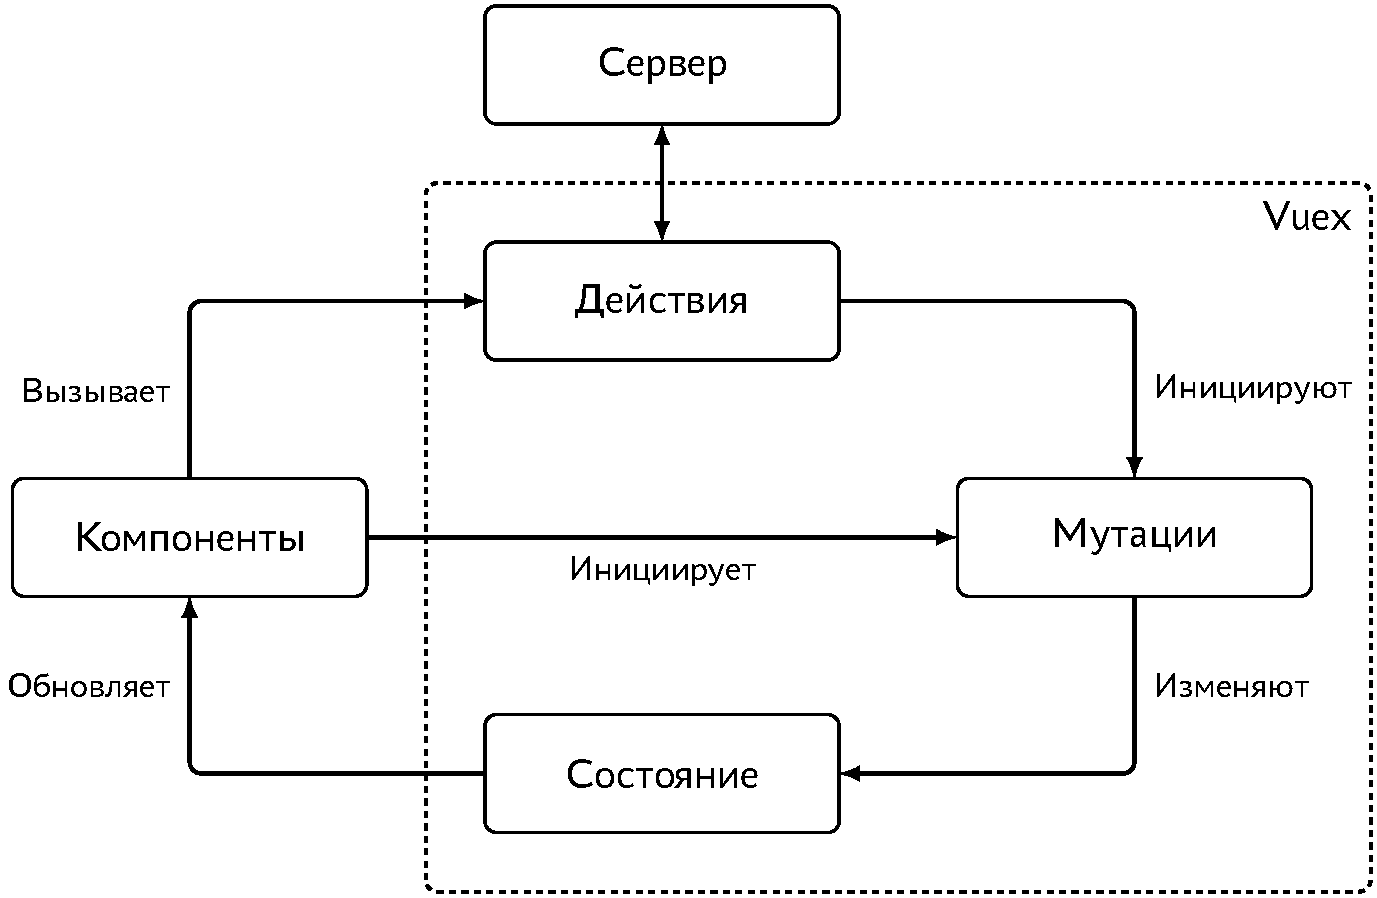
\includegraphics[width=.9\textwidth]{img/tikz/vuex-oneway-data-flow/pic}
  \vspace*{12pt}
  \caption{Однонаправленный поток данных при использовании Vuex}\label{fig:vuex-oneway-data-flow}
\end{figure}


\subsubsection{Модули хранилища данных}

Глобальные данные о~состоянии приложения по умолчанию хранятся в~одном и~том же объекте. Рост числа модулей приложения неизбежно приводит к~тому, что структура данного объекта существенно усложняется, а~именование мутаций и~действий может вызывать затруднения из-за требования к~уникальности имён сущностей Vuex.

Для решения описанных выше проблем Vuex предоставляет инструменты для разделения хранилища на \emph{модули}. Модули представляют из себя самостоятельные части глобального состояния, каждая из которых может содержать объект с~данными, мутации и~т.д. При использовании данного подхода возможные проблемы с~именованием решаются благодаря тому, что каждый модуль Vuex может иметь собственное пространство имён.

% TODO Добавить пример работы с модулями

Хранилище Vuex, используемое в разрабатываемом приложении, было разделено на модули, соответствующие важнейшим подсистемам программного обеспечения устройств Reach и~Reach~RS:
\begin{dashitemize}
  \item информация о~текущей версии приложения, а~также об устройстве и его конфигурация (модули \emph{device} и~\emph{settings});
  \item позиционирование и~режим RTK (модуль \emph{status});
  \item входящие и~исходящие потоки данных (модуль \emph{streams});
  \item беспроводные соединения (модуль \emph{wireless});
  \item изыскания (модуль \emph{survey});
  \item состояние компонентов графического интерфейса (модуль \emph{ui}).
\end{dashitemize}

Схема модулей глобального хранилища изображена на рисунке \ref{fig:vuex-modules}.

\begin{figure}[h!]
  \centering
  \setlength{\fboxsep}{5pt}
  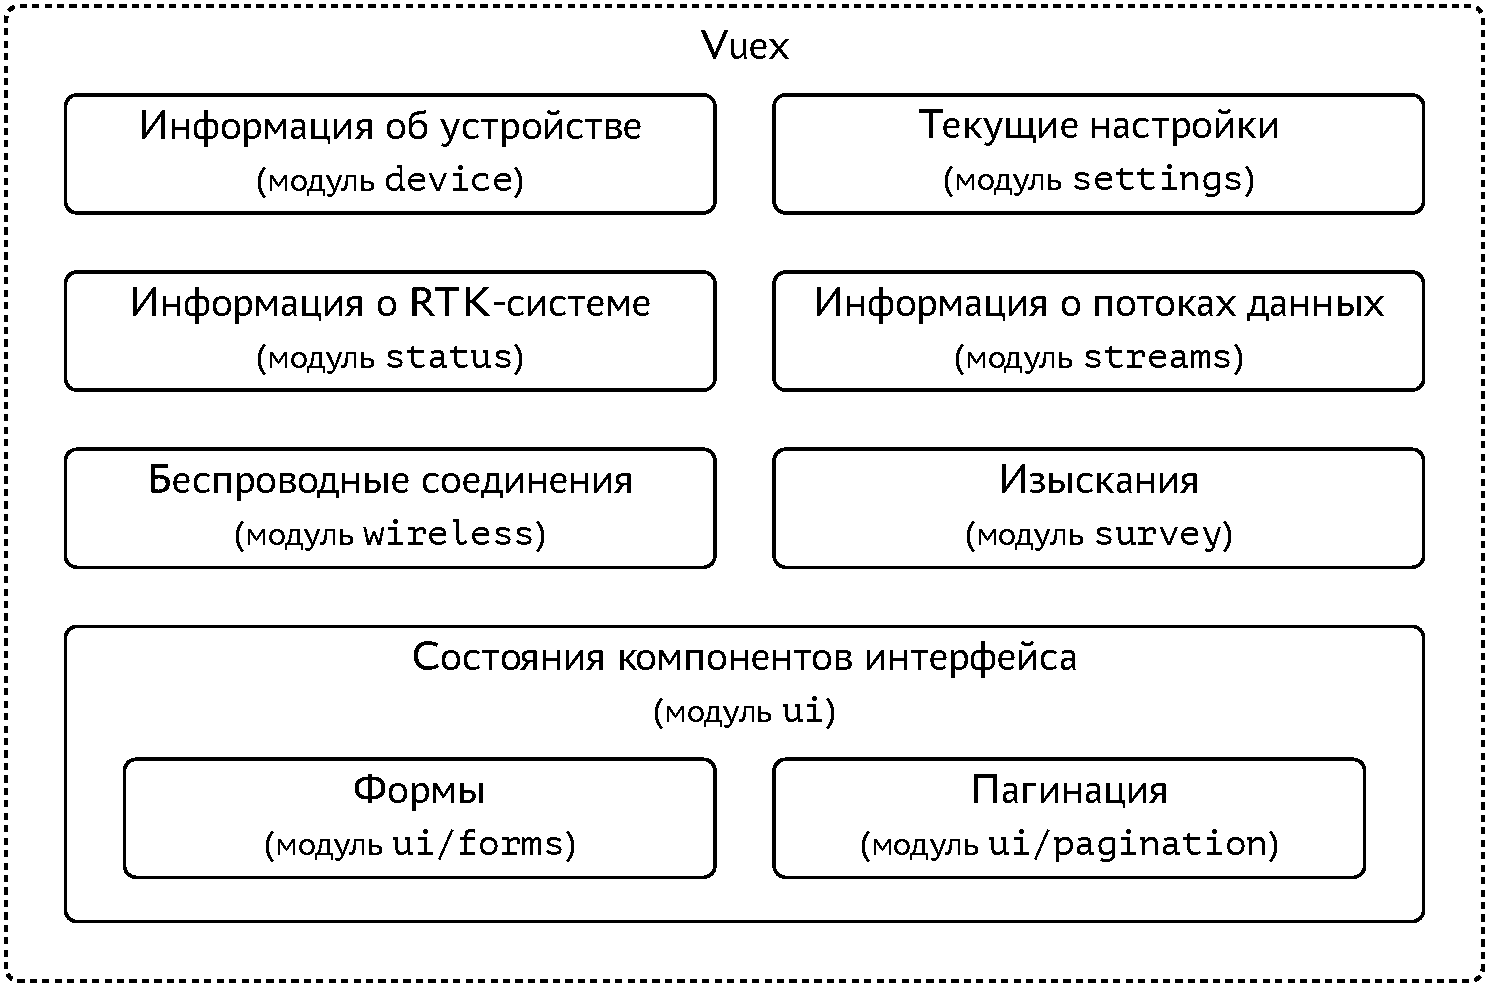
\includegraphics[width=.9\textwidth]{img/tikz/vuex-modules/pic}
  \vspace*{6pt}
  \caption{Модульная структура хранилища Vuex}\label{fig:vuex-modules}
\end{figure}



\subsection{Модули и~компоненты приложения}

Далее описана структура и~организация модулей и~компонентов разрабатываемого веб-приложения. Первые два пункта посвящены модулям общего назначения и~вспомогательным компонентам, которые необходимы для создания моделей представления, описанных в~подразделе \ref{subsec:app-modules-requirements}. Сами же модели представления описаны в~третьем пункте текущего подраздела.


\subsubsection{Модули общего назначения}

К~модулям общего назначения относятся модуль работы с~картами и~модуль обработки событий. Рассмотрим каждый из их подробнее.

\paragraph{Модуль работы с~картами}

Модуль работы с~картами представляет из себя обёртку (англ. \emph{wrapper}) над частью библиотеки OpenLayers, используемой в~разрабатываемом приложении для отображения карт и различной информации на них. Код модуля содержится в~файле \emph{olWrapper.js}.

\newpage

Данный модуль предназначен для повышения удобства создания однотипных карт -- для добавления карты на страницу достаточно импортировать модуль в~код приложения и~вызвать соответствующие функции.

Импорт необходимых модулей OpenLayers, единожды осуществляемый в~модуле работы с~картами (см.~листинг \ref{lst:modules__maps__imports}), исключает повторение существенного количества строк кода.

\lstinputlisting[
  caption={olWrapper.js: импорт необходимых модулей OpenLayers},
  label={lst:modules__maps__imports}
]{src/modules__maps__imports.js}

% TODO Добавить полный листинг в Приложения


\paragraph{Модуль обработки событий}

Модуль обработки событий (\emph{eventsModule.js}) выполняет ряд ключевых задач, необходимых для работы приложения:
\begin{dashitemize}
  \item инициализация WebSocket-подключения;
  \item обработка разрыва (восстановления) соединения с сервером;
  \item оповещение пользователя о различных событиях.
  \item инициализация модулей Vuex путём вызова их действий.
\end{dashitemize}

В листинге \ref{lst:modules__events__short} представлено содержимое файла eventsModule.js (полный листинг файла см. в приложении ??). По умолчанию модуль экспортирует функцию, выполнение которой зарегистрирует несколько слушателей событий Socket.IO и вызовет действие \emph{<<activate>>} (\emph{activate} с англ. -- <<активировать>>) в четырёх модулях Vuex.

Действия с названием <<activate>> присутствуют во всех модулях Vuex, кроме модулей, отвечающих за хранение состояния компонентов интерфейса (см. рис.~\ref{fig:vuex-modules}). <<Активация>> модуля Vuex подразумевает под собой:
\begin{dashitemize}
  \item установку значений по умолчанию в объекте состояния (при необходимости);
  \item регистрацию слушателей определённых широковещательных сообщений сервера;
  \item отправку на сервер запросов на получение данных;
  \item создание таймеров для периодических опросов сервера.
\end{dashitemize}

\lstinputlisting[
  caption={Модуль обработки событий},
  label={lst:modules__events__short}
]{src/modules__events__short.js}

Также модуль обработки событий экспортирует объект \emph{socket}, импортируя который, любой компонент приложения сможет осуществлять общение с сервером через WebSocket-события.


\subsubsection{Вспомогательные компоненты}

Вспомогательные компоненты представляют из себя набор блоков и элементов интерфейса, необходимых для создания всевозможных представлений приложения. Данные компоненты включают в себя кнопки, переключатели, панели, индикаторы выполнения и т.д. (см. рис.~\ref{fig:common-components}).

\begin{figure}[h!]
  \centering
  \setlength{\fboxsep}{5pt}
  \subfloat[\label{sub:common-components__buttons}]{
    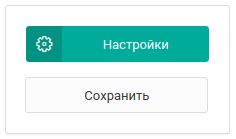
\includegraphics[height=4cm]{img/buttons}
  }\\
  \subfloat[\label{sub:common-components__toggles}]{
    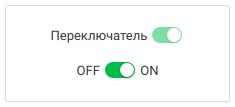
\includegraphics[height=3.25cm]{img/togglers}
  }
  \vspace*{6pt}
  \caption{
    Пример вспомогательных компонентов:\\
    \protect\subref{sub:common-components__buttons} - кнопки,
    \protect\subref{sub:common-components__toggles} - переключатели
  }
  \label{fig:common-components}
\end{figure}

Каждый вспомогательный элемент является Vue-компонентом, что даёт возможность управлять внешним видом, содержимым и поведением каждого из них. К примеру, компонент <<переключатель>> (англ. \emph{toggle}) кроме обязательного параметра, являющегося булевой переменной, также позволяет настроить свой текст, цвет и доступность для изменения состояния (см. листинг~\ref{lst:component__common__toggle__short}).

\newpage

\lstinputlisting[
  caption={Настраиваемые свойства компонента <<переключатель>>},
  label={lst:component__common__toggle__short}
]{src/component__common__toggle__short.vue}


\subsubsection{Модели представления и представления}

\paragraph{Статус}

<<Статус>> является представлением, отображаемым по умолчанию. Основная задача данного представления -- вывод информации об RTK-системе, сигналах спутников и позиции приёмника.

<<Статус>> зависит от данных, содержащихся в модуле status хранилища Vuex. Модуль status содержит всю необходимую для вывода информацию, обновляемую в режиме реального времени благодаря реактивности Vuex и зарегистрированным слушателям широковещательных сообщений сервера.

На рисунке \ref{fig:status-detailed} изображена страница <<Статус>>, отображающая состояние ровера, получающего поправки с~базы. Набор элементов страницы и их отображение меняется, в зависимости от наличия (отсутствия) тех или иных данных, а~также от режима работы RTKLIB. Так, например, столбчатая диаграмма значений соотношений сигнал/шум для принимаемых со спутников сигналов примет вид, изображённый на рисунке \ref{fig:status-snr-rover}, при отсутствии данных о~спутниках, видимых базе. Другим примером может служить скрытие информации о~позиции базы и~RTK-параметрах при переводе RTKLIB в~режим Single (см. пункт \ref{subsec:rtklib-modes}).

% TODO Сделать нормальную картинки
\begin{figure}[h!]
  \centering
  \setlength{\fboxsep}{5pt}
  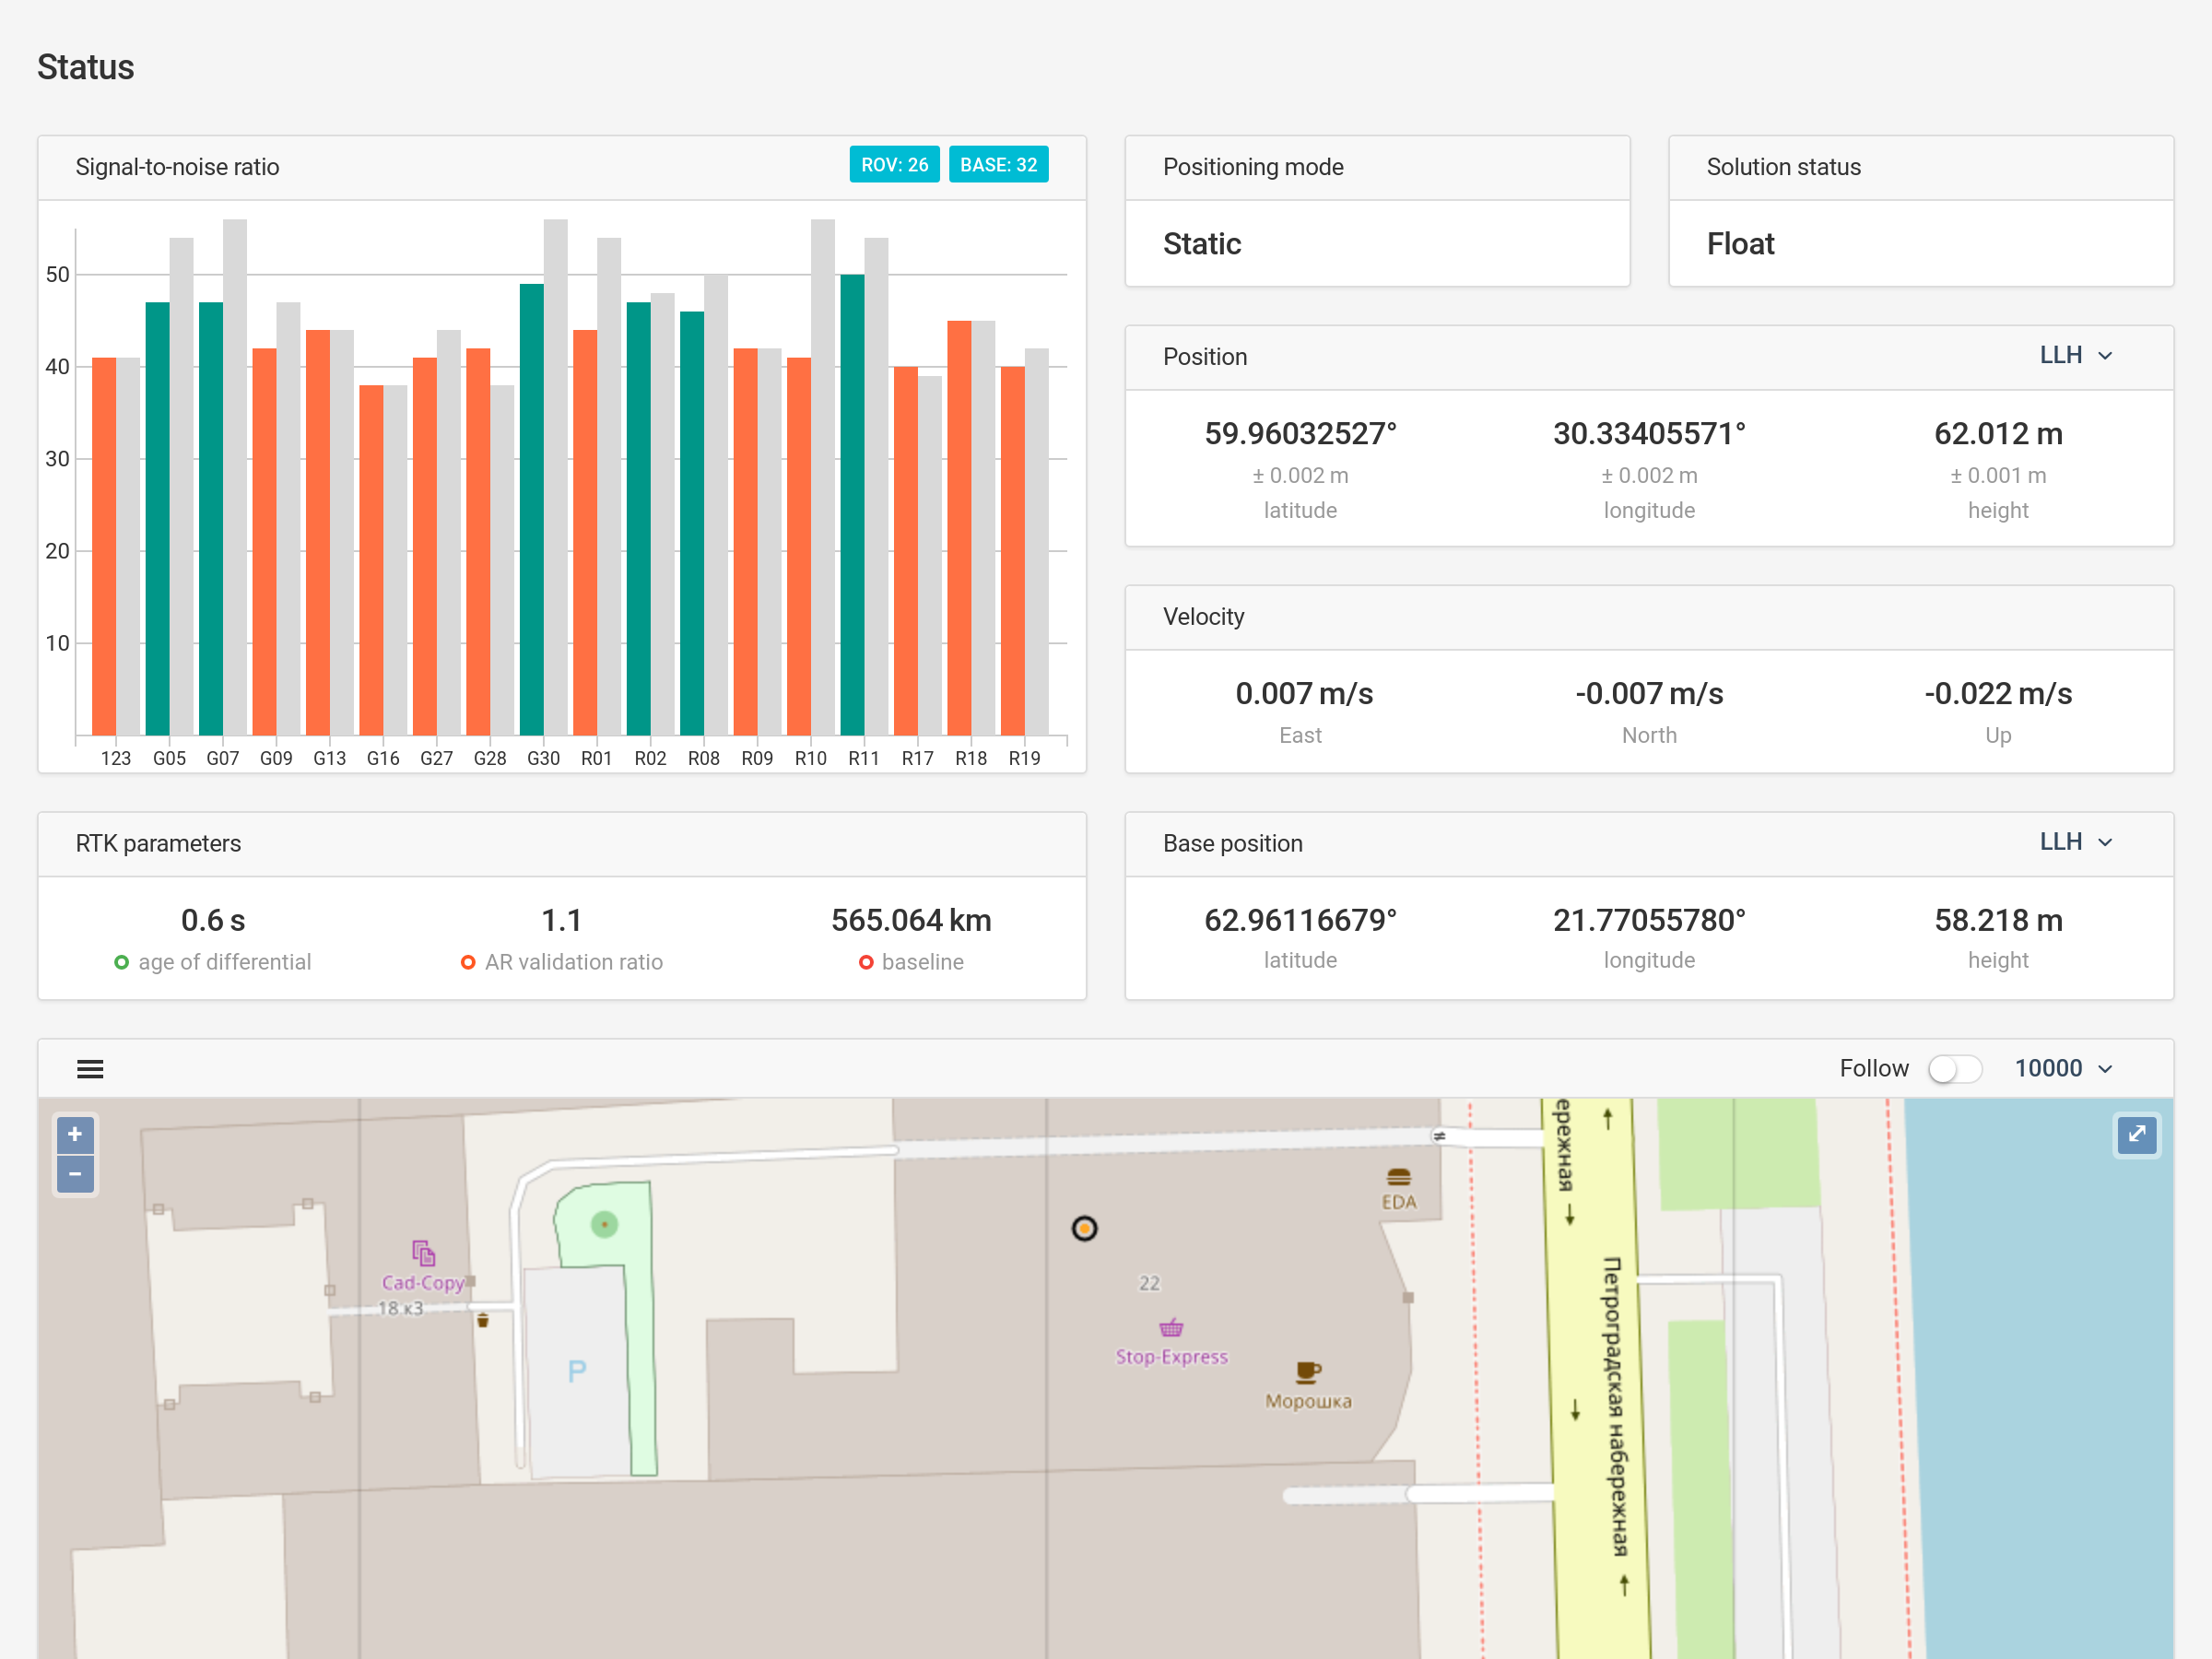
\includegraphics[width=.9\textwidth]{img/reachview/status_content_laptop}
  \vspace*{6pt}
  \caption{Страница <<Статус>>}
  \label{fig:status-detailed}
\end{figure}

\begin{figure}[h!]
  \centering
  \setlength{\fboxsep}{5pt}
  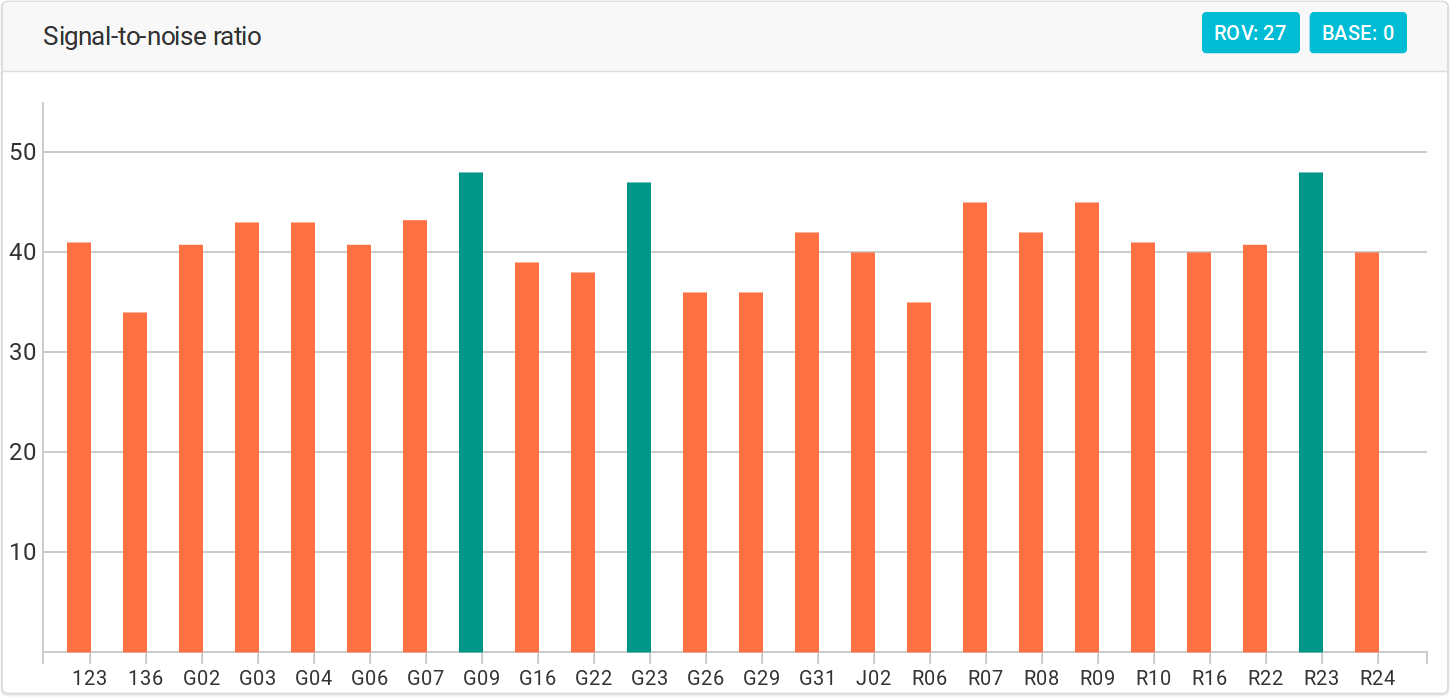
\includegraphics[width=.9\textwidth]{img/reachview/status_snr_rover}
  \vspace*{6pt}
  \caption{Отсутствие данных о спутниках, видимых базе}
  \label{fig:status-snr-rover}
\end{figure}

\paragraph{Изыскания}

<<Изыскания>> -- раздел приложения, с~помощью которого происходит основная часть работы с~устройством. Используя данный интерфейс пользователь может производить геодезические изыскания -- сбор точек на местности, с~разделением их на проекты.

В~соответствии с требованиями, перечисленными в~пункте \ref{subsec:survey-requirements}, был разработан модуль приложения, основанный на сущностях и~прецедентах, описанных на рисунках \ref{fig:survey-uml-classes} и~\ref{fig:survey-uml-usecase} соответственно.

\begin{figure}[h!]
  \centering
  \setlength{\fboxsep}{5pt}
  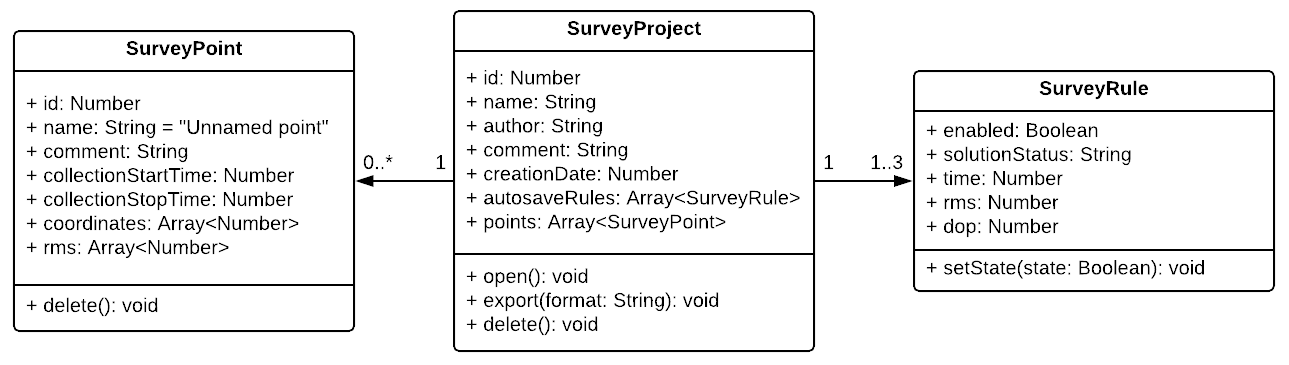
\includegraphics[width=\textwidth]{img/uml/survey_class}
  \caption{Диаграмма классов модуля <<Изыскания>>}
  \label{fig:survey-uml-classes}
\end{figure}

\begin{figure}[h!]
  \centering
  \setlength{\fboxsep}{5pt}
  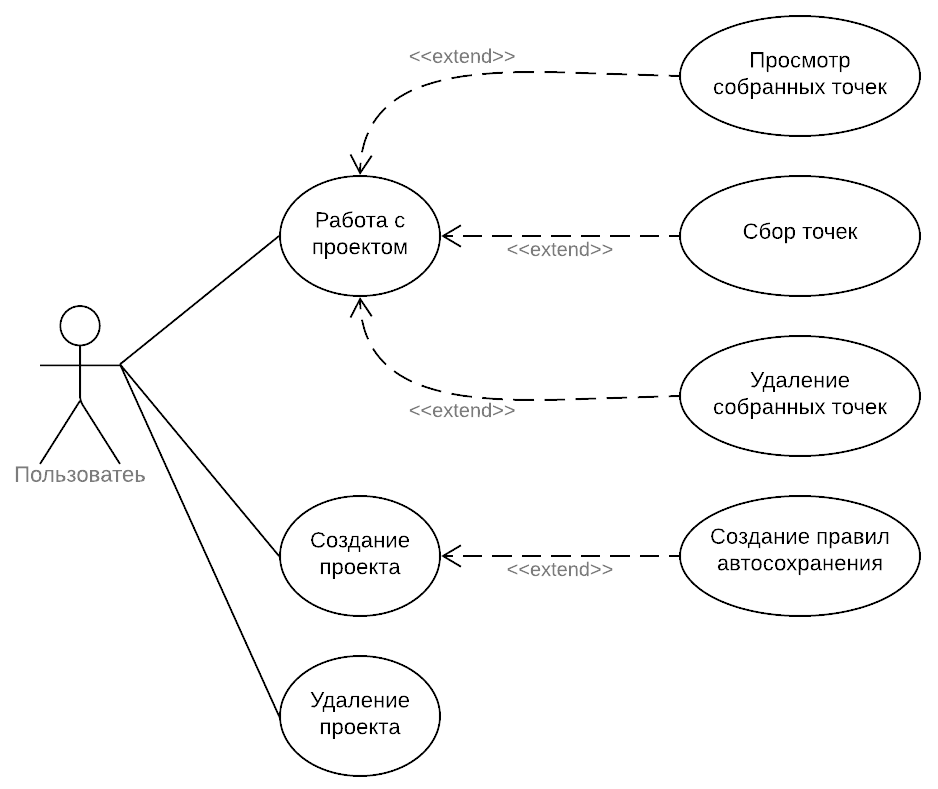
\includegraphics[width=.8\textwidth]{img/uml/survey_usecase}
  \vspace*{6pt}
  \caption{Диаграмма прецедентов модуля <<Изыскания>>}
  \label{fig:survey-uml-usecase}
\end{figure}

Модуль <<Изыскания>> состоит из множества отдельных представлений, переключаясь между которыми, пользователь осуществляет разнообразные действия с~собранными данными. Одной из основных задач при разработке данного модуля было чёткое описание возможных состояний и~условий перехода между ними. На рисунке \ref{fig:survey-uml-state} представлена диаграмма состояний модуля <<Изыскания>>.

\begin{figure}[h!]
  \centering
  \setlength{\fboxsep}{5pt}
  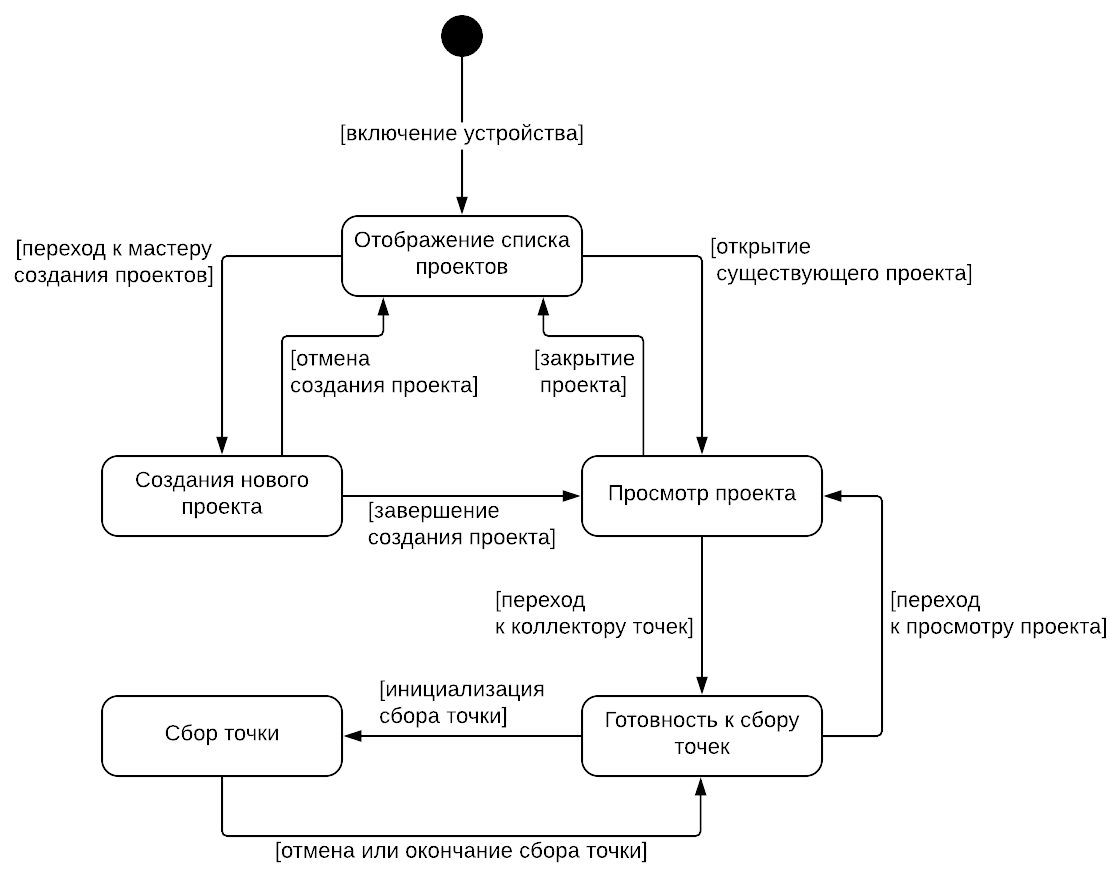
\includegraphics[width=.8\textwidth]{img/uml/survey_state}
  \caption{Диаграмма состояний модуля <<Изыскания>>}
  \label{fig:survey-uml-state}
\end{figure}

\paragraph{Модули настройки параметров работы устройства}
\label{subsec:device-settings}

К модулям, предназначенным для настройки параметров устройства, относятся <<Настройки RTK>> и~<<Управление камерой>>. Представления данных модулей (рисунки \ref{fig:rtk-settings} и~\ref{fig:camera-control}) реализованы в~виде форм настроек, отображающих требования описанные в~пункте \ref{subsec:survey-requirements}.

\begin{figure}[h!]
  \centering
  \setlength{\fboxsep}{5pt}
  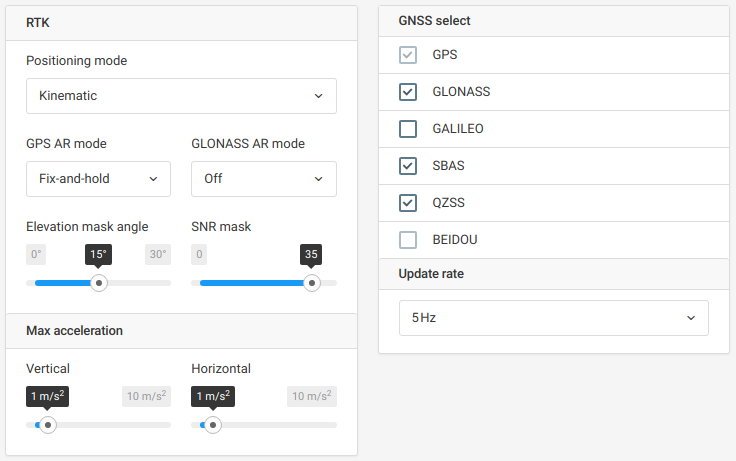
\includegraphics[width=.8\textwidth]{img/reachview/rtk-settings}
  \vspace*{6pt}
  \caption{Формы вкладки <<Настройки RTK>>}
  \label{fig:rtk-settings}
\end{figure}

\begin{figure}[h!]
  \centering
  \setlength{\fboxsep}{5pt}
  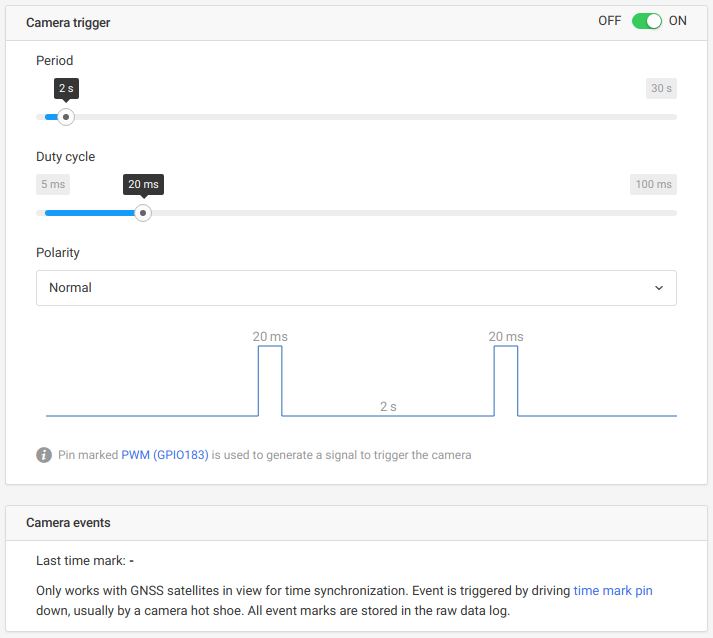
\includegraphics[width=.8\textwidth]{img/reachview/camera-control__cut}
  \vspace*{6pt}
  \caption{Формы вкладки <<Управление камерой>>}
  \label{fig:camera-control}
\end{figure}

Алгоритм применения новых настроек с~помощью форм вкладок <<Настройки RTK>> и~<<Управление камерой>> представлен на рисунке \ref{fig:basic-form-apply}. В алгоритме отсутствует этап валидации применяемой конфигурации, т.к. формы рассматриваемых вкладок не содержат полей, подразумевающих ввод произвольных пользовательских значений.

\begin{figure}[h!]
  \centering
  \setlength{\fboxsep}{5pt}
  \includegraphics[width=.75\textwidth]{example-image}
  \vspace*{6pt}
  \caption{Схема алгоритма применения настроек с~помощью графической формы}
  \label{fig:basic-form-apply}
\end{figure}

\paragraph{Модули настройки входящих и исходящих потоков данных}

За настройку входящих и исходящих потоков данных отвечают модули <<Входящие поправки>>, <<Выдача позиции>> и <<Режим базы>> (рисунки ??, ?? и ?? соответственно). Как и в случае с компонентами, описанными в подпункте \ref{subsec:device-settings}, представления рассматриваемых модулей содержат исключительно формы настроек.

\begin{figure}[h!]
  \centering
  \setlength{\fboxsep}{5pt}
  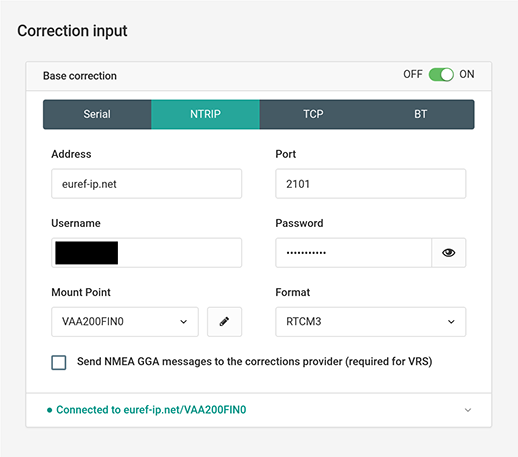
\includegraphics[width=.5\textwidth]{img/reachview/correction-input_content_laptop}
  \vspace*{6pt}
  \caption{Формы вкладки <<Входящие поправки>>}
  \label{fig:correction-input}
\end{figure}

\begin{figure}[h!]
  \centering
  \setlength{\fboxsep}{5pt}
  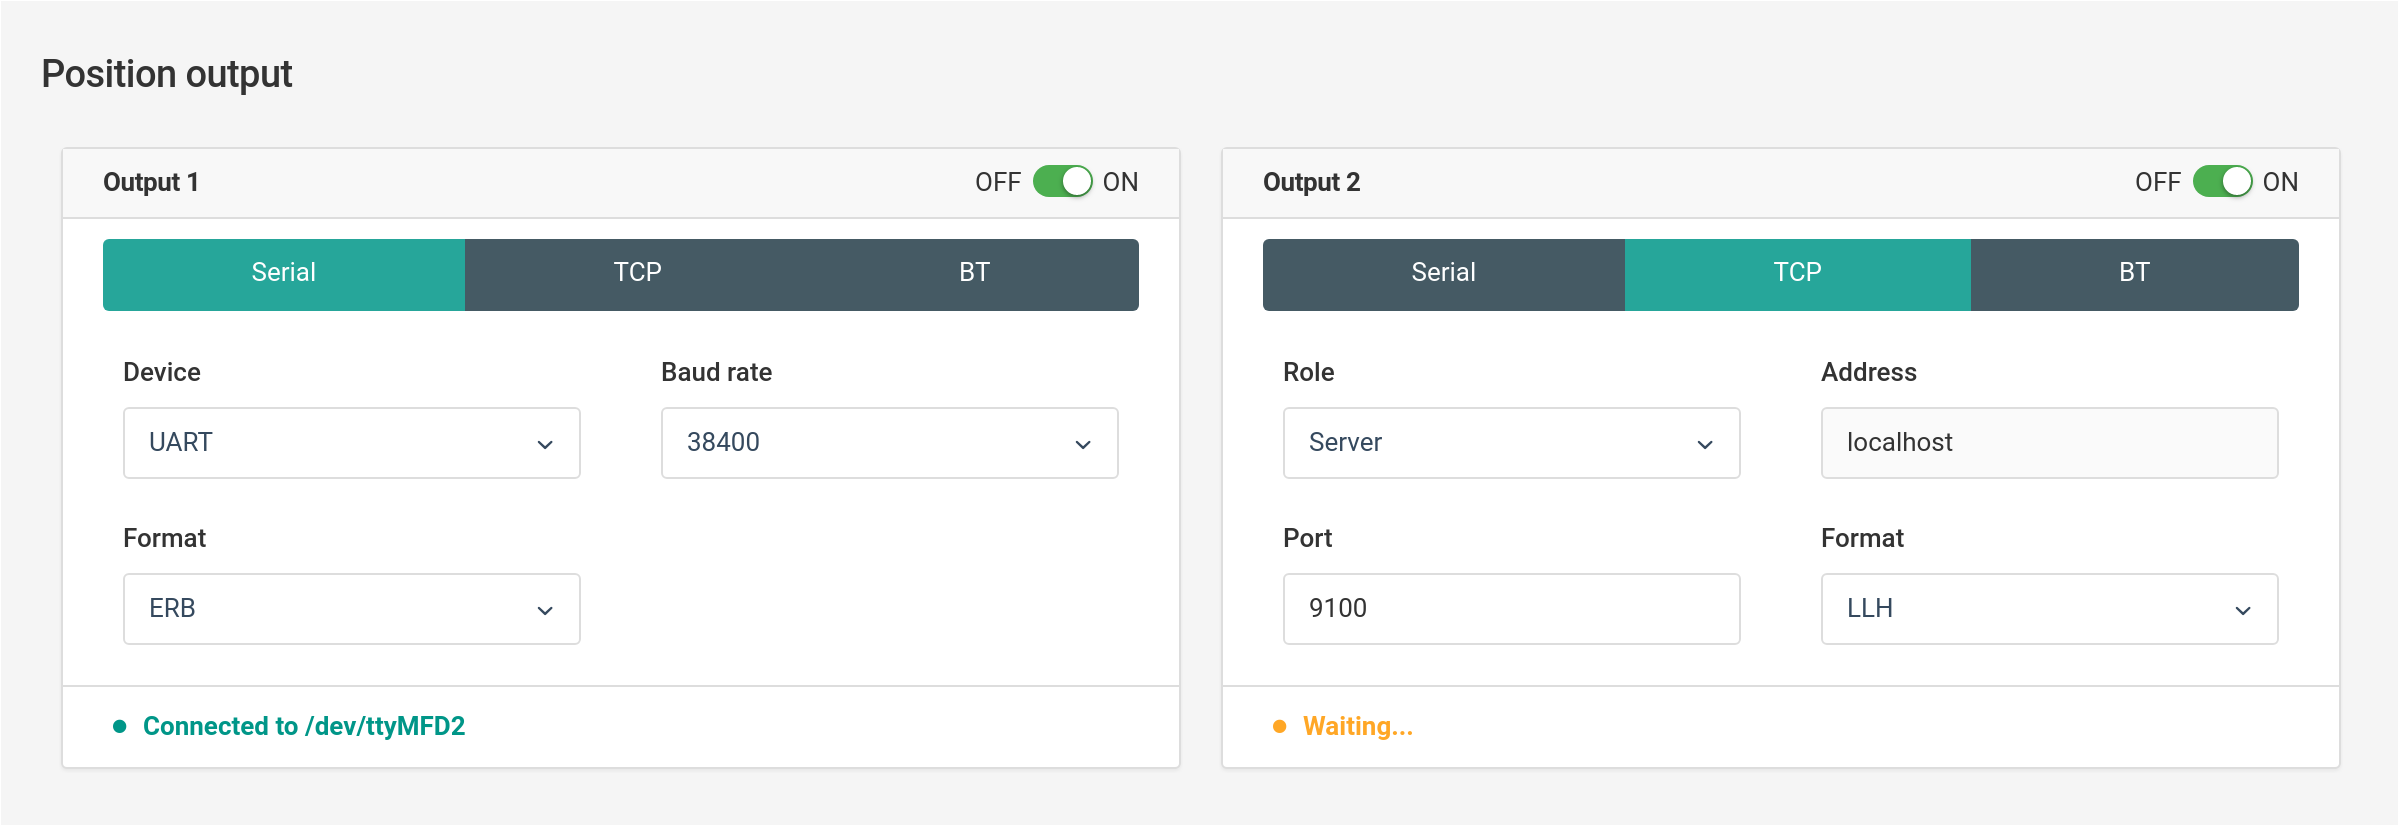
\includegraphics[width=.8\textwidth]{img/reachview/position-output_content_laptop}
  \vspace*{6pt}
  \caption{Формы вкладки <<Выдача позиции>>}
  \label{fig:position-output}
\end{figure}

\begin{figure}[h!]
  \centering
  \setlength{\fboxsep}{5pt}
  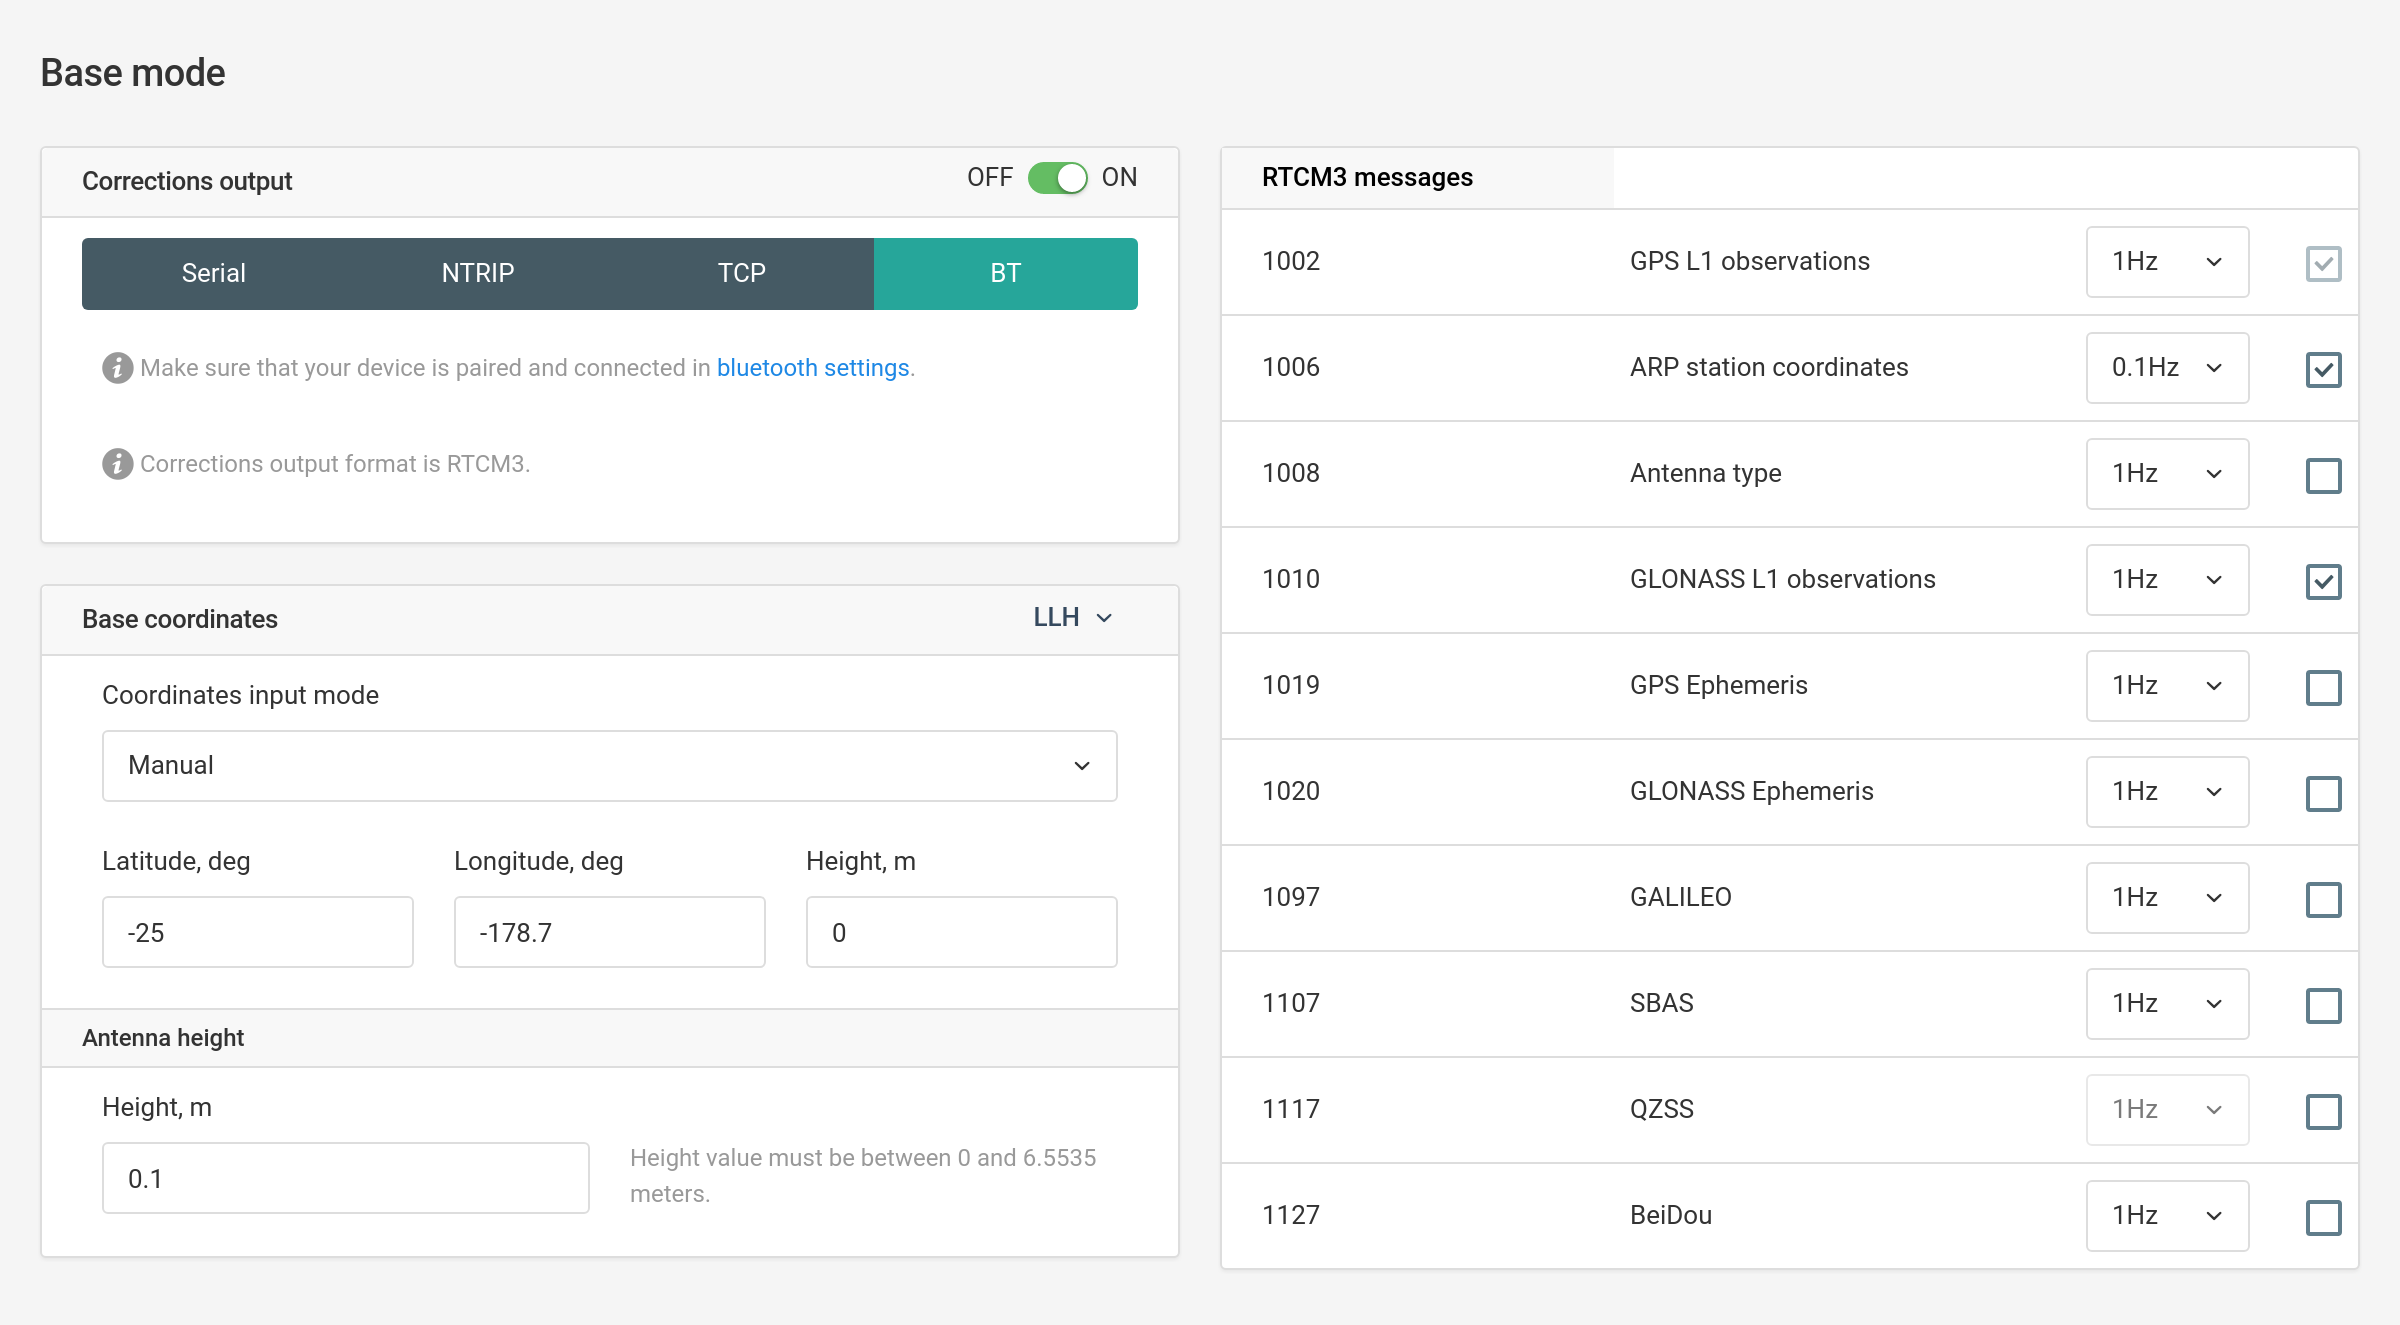
\includegraphics[width=.8\textwidth]{img/reachview/base-mode_content_laptop}
  \vspace*{6pt}
  \caption{Формы вкладки <<Режим базы>>}
  \label{fig:base-mode}
\end{figure}

Отличительными особенностями форм представлений модулей настройки потоков данных являются:
\begin{dashitemize}
  \item необходимость валидации значений, введённых пользователем;
  \item необходимость проверки наличия возможных конфликтов, описанных в пункте \ref{subsec:general-io-restrictions}.
\end{dashitemize}

С учётом описанных особенностей, алгоритм применения настроек потоков данных с помощью графических форм принимает вид, представленный на рисунке \ref{fig:io-form-apply}.

\begin{figure}[h!]
  \centering
  \setlength{\fboxsep}{5pt}
  \includegraphics[width=.75\textwidth]{example-image}
  \vspace*{6pt}
  \caption{Схема алгоритма применения настроек потоков данных с~помощью графической формы}
  \label{fig:io-form-apply}
\end{figure}

\paragraph{Модули настройки беспроводных соединений}

Модули настройки беспроводных соединений -- <<Wi-Fi>> и <<Bluetooth>> (рисунки ?? и ??) -- отвечают за подключение приёмника к сетям Wi-Fi и за его сопряжение другими устройствами.

Модули реализованы в соответствии с требованиями, описанными в пункте \ref{subsec:survey-requirements}. Диаграммы вариантов использования вкладок <<Wi-Fi>> и <<Bluetooth>> представлены на рисунках ?? и ?? соответственно.

\paragraph{Логирование}

<<Логирование>> -- модуль приложения, с помощью которого пользователь получает доступ к управлению логами данных приёмника.

Представление модуля (см. рис.~??) состоит из трёх панелей для управления процессом записи логов (доступны логи данных трёх типов) и списка доступных логов, разделённых по дате начала записи.

Диаграмма вариантов использования вкладки <<Логирование>> представлена на рисунке ??.

\paragraph{Общие настройки}

Модуль предоставляет пользователю доступ к ряду общих настроек  утилитарных функций приёмника (см. пункт \ref{subsec:settings-module}).

Возможности, доступные во вкладке <<Общие настройки>>, описаны с помощью диаграммы прецедентов, изображённой на рисунке ??.



\subsection{Тестирование приложение}


\subsubsection{Модульное тестирование}

В ходе разработки исходный код приложения был покрыт модульными тестами. Для написания тестов были использован следующие инструменты:
\begin{dashitemize}
  \item \textbf{Karma} [?] -- утилита для запуска JavaScript-тестов;
  \item \textbf{Mocha} [?] -- тестовый фреймворк для JavaScript-приложений;
  \item \textbf{Istanbul} [?] -- утилита для анализа покрытия исходного кода JavaScript-приложений модульными тестами.
\end{dashitemize}

В листинге ?? представлен пример объявления тестовых случаев (англ. \emph{test case}) и тестовых наборов (англ. \emph{test suite}).

{\color{gray}{*listing*}}

На рисунке \ref{fig:karma-output} продемонстрирован пример вывода Karma, работающей с Istanbul.

\begin{figure}[h!]
  \centering
  \setlength{\fboxsep}{5pt}
  \fbox{
    \parbox{.9\textwidth}{
      {
        \footnotesize\ttfamily
        \$ npm run test \\

        ...\\

        Executed 148 of 154 (skipped 6) SUCCESS (6.701 secs / 5.888 secs) \\
        TOTAL: 148 SUCCESS \\

        ========================== Coverage summary ==========================\\
        Statements~: 58.99\% ( 1109/1880 )\\
        Branches~~~: 51.66\% ( 606/1173 )\\
        Functions~~: 47.92\% ( 115/240 )\\
        Lines~~~~~~: 59.58\% ( 1088/1826 )\\
        ======================================================================
    }}
  }
  \vspace*{6pt}
  \caption{Запуск тестов с помощью утилиты Karma}
  \label{fig:karma-output}
\end{figure}


\subsubsection{Функциональное тестирование}

Функциональное тестирование приложения проводилось в ручном и автоматизированном режимах. Для автоматизации тестов были использованы язык программирования Python и библиотека Selenuim [?], позволяющая автоматизировать управление веб-браузерами (см. листинг ??).

Благодаря использованию тестового фреймворка pytest, предназначенного для написание тестов на Python, был автоматизирован процесс тестирования приложения в нескольких браузерах. Вызов графического сервера Xvfb [?] из кода Python-тестов позволил добавить возможность проверки приложения на различных разрешениях экрана.

{\color{gray}{*listing*}}



\subsection{Выводы по разделу 3}

\begin{dashitemize}
  \item Исходя из выбранных инструментов, было создано окружение для разработки, которое позволило использовать новейшие веб-технологии при создании приложения.
  \item Было создано кроссбраузерное, адаптивное веб-приложение для управления устройствами Reach и Reach~RS, которое соответствует всем заявленным требованиям (см. рис.~??).
  \item Для разработанного приложения были созданы комплексы модульных и функциональных тестов, позволяющие автоматизировать проверку работы как отдельных компонентов, так и всего приложения в целом.
\end{dashitemize}

\begin{figure}[h!]
  \centering
  \setlength{\fboxsep}{5pt}
  \subfloat[\label{sub:status-responsive__lg}]{
    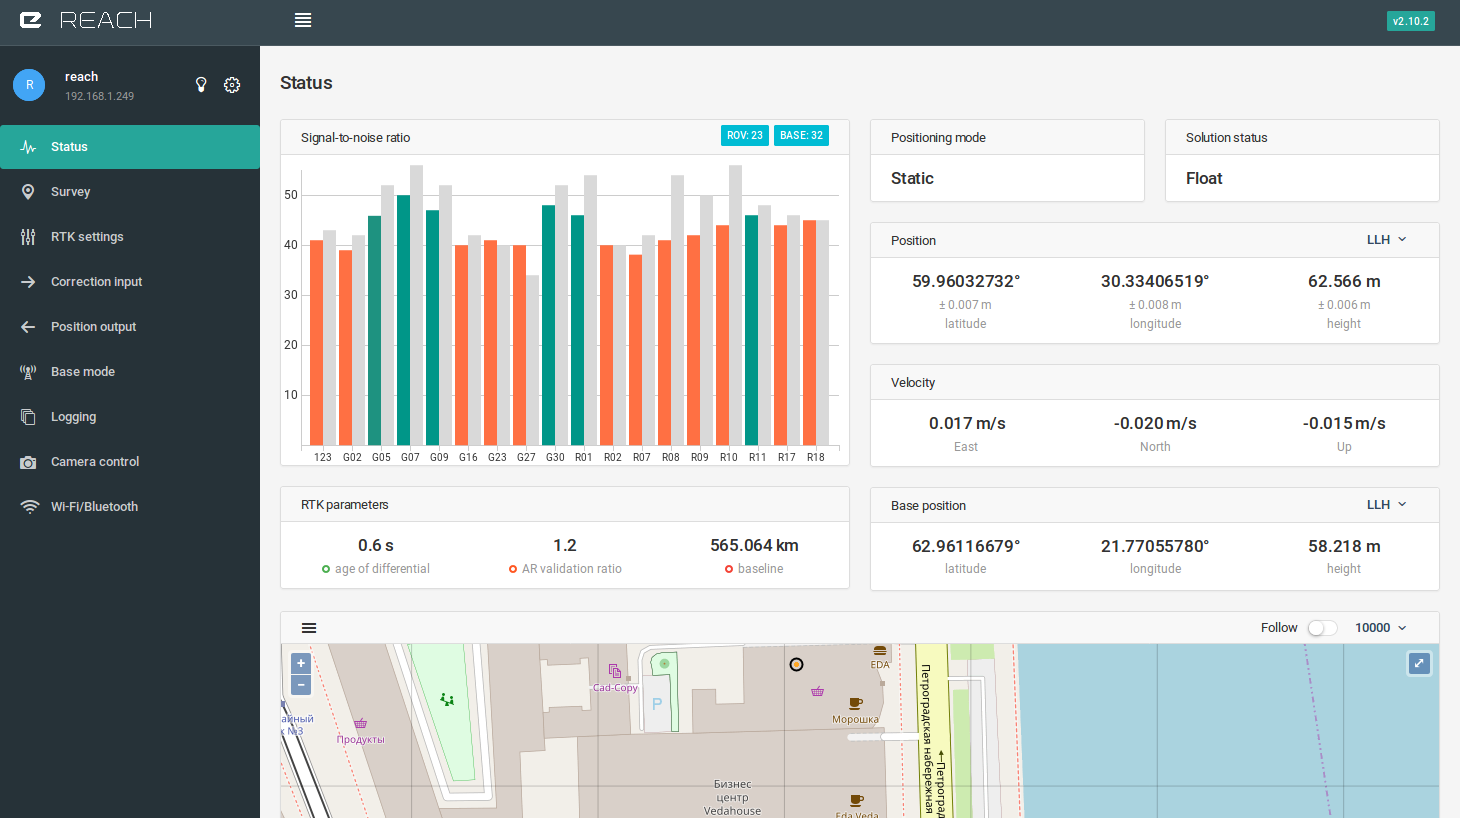
\includegraphics[width=.9\textwidth]{img/reachview/home}
  }\\
  \subfloat[\label{sub:status-responsive__xs}]{
    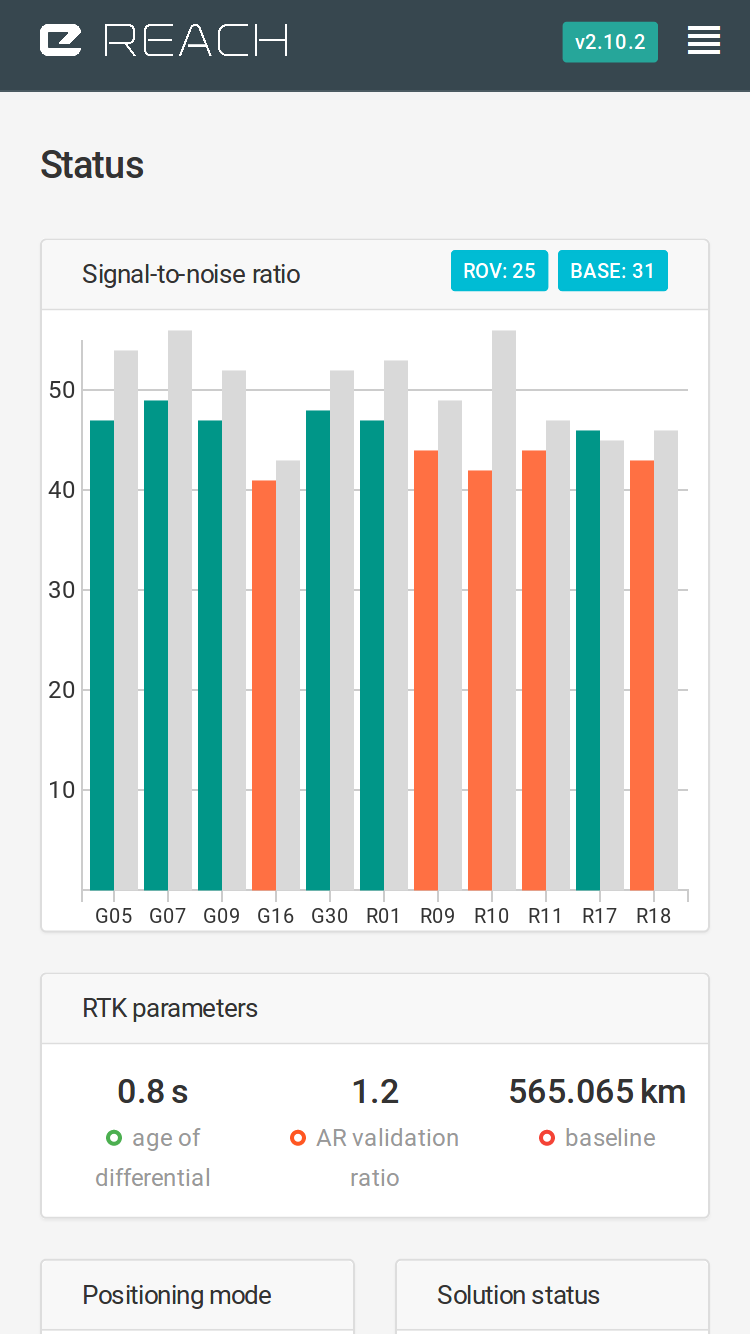
\includegraphics[width=.45\textwidth]{img/reachview/homepage_responsive-xs}
  }
  \vspace*{6pt}
  \caption{
    Адаптация приложения к~размеру дисплея устройства\\(на примере страницы <<Статус>>):
    \protect\subref{sub:status-responsive__lg} - экран ноутбука,
    \protect\subref{sub:status-responsive__xs} - экран смартфона
  }
  \label{fig:status-responsive}
\end{figure}

\newpage
